%% 
%% Copyright 2007, 2008, 2009 Elsevier Ltd
%% 
%% This file is part of the 'Elsarticle Bundle'.
%% ---------------------------------------------
%% 
%% It may be distributed under the conditions of the LaTeX Project Public
%% License, either version 1.2 of this license or (at your option) any
%% later version.  The latest version of this license is in
%%    http://www.latex-project.org/lppl.txt
%% and version 1.2 or later is part of all distributions of LaTeX
%% version 1999/12/01 or later.
%% 
%% The list of all files belonging to the 'Elsarticle Bundle' is
%% given in the file `manifest.txt'.
%% 
%% Template article for Elsevier's document class `elsarticle'
%% with harvard style bibliographic references
%% SP 2008/03/01

%%\documentclass[preprint,12pt,authoryear]{elsarticle}

%% Use the option review to obtain double line spacing
%% \documentclass[authoryear,preprint,review,12pt]{elsarticle}

%% Use the options 1p,twocolumn; 3p; 3p,twocolumn; 5p; or 5p,twocolumn
%% for a journal layout:
%% \documentclass[final,1p,times,authoryear]{elsarticle}
%% \documentclass[final,1p,times,twocolumn,authoryear]{elsarticle}
%% \documentclass[final,3p,times,authoryear]{elsarticle}
\documentclass[final,3p,times,twocolumn,authoryear]{elsarticle}
%% \documentclass[final,5p,times,authoryear]{elsarticle}
%% \documentclass[final,5p,times,twocolumn,authoryear]{elsarticle}

%% For including figures, graphicx.sty has been loaded in
%% elsarticle.cls. If you prefer to use the old commands
%% please give \usepackage{epsfig}

%% The amssymb package provides various useful mathematical symbols
\usepackage{amssymb}
%% The amsthm package provides extended theorem environments
%% \usepackage{amsthm}

\usepackage[utf8]{inputenc} % Codificacao do documento (conversão automática dos acentos)

%% The lineno packages adds line numbers. Start line numbering with
%% \begin{linenumbers}, end it with \end{linenumbers}. Or switch it on
%% for the whole article with \linenumbers.
%% \usepackage{lineno}

\journal{IAA CubeSat 2016}

\begin{document}

\begin{frontmatter}
%% Title, authors and addresses

%% use the tnoteref command within \title for footnotes;
%% use the tnotetext command for theassociated footnote;
%% use the fnref command within \author or \address for footnotes;
%% use the fntext command for theassociated footnote;
%% use the corref command within \author for corresponding author footnotes;
%% use the cortext command for theassociated footnote;
%% use the ead command for the email address,
%% and the form \ead[url] for the home page:
%% \title{Title\tnoteref{label1}}
%% \tnotetext[label1]{}
%% \author{Name\corref{cor1}\fnref{label2}}
%% \ead{email address}
%% \ead[url]{home page}
%% \fntext[label2]{}
%% \cortext[cor1]{}
%% \address{Address\fnref{label3}}
%% \fntext[label3]{}

\title{Electrical Power System}

%% use optional labels to link authors explicitly to addresses:
 \author{A.A.Viana J\'{u}nior, O.M.Petito, T.A.D.O.Cordeiro}
 \address{Escola de Engenharia Mauá, São Caetano do Sul, Brasil}
 \address{Escola de Engenharia Mauá, São Caetano do Sul, Brasil}
 \address{Escola de Engenharia Mauá, São Caetano do Sul, Brasil}

%\author{}

%\address{}

\begin{abstract}

	This work is discusses the development of a power system capable of supplying the entire energy demand of the attitude control subsystem, communication, data processing and payload of the CubeSat project of the Escola de Engenharia Mauá. The power system developed is responsible for generating, distribution and control of the entire energy flow of the CubeSat Mauá. The energy generated by high efficiency aerospace photocells, endowed with the triple junction technology (GaInP/GaAs/Ge) is stored in Ion-Lithium batteries. The distribution of energy is made by three levels of stabilized voltages and regulated in 3,3V, 5V and 12V, plus a unregulated level supplied directly from the battery. In case of failure, a set of redundant power supplies are able to take any of the levels of regulated voltages. All control of the power system is performed by a microcontroller, which collects and analyzes data, such as temperature, voltage and current to determine whether the system power will come from major sources or from redundant ones. Through a CAN network, the microcontroller transmits telemetry information to a Data Processing Unit which takes more complex decisions involving all the CubeSat subsystems.

\end{abstract}

\begin{keyword}
 
	EPS, power system, CubeSat, power management.

\end{keyword}

\end{frontmatter}

%% \linenumbers

%% main text
\section{Objective}
\label{Objective}

	Esse projeto, fez parte do projeto de desenvolvimento do CubeSat do NSEE-IMT da Escola de Engenharia Mauá, visou fornecer a energia necessária, com incidência direta ou não de luz solar, para garantir o sucesso de missões espaciais.

\section{Topology}
\label{Topologia}

	A topologia do circuito foi o passo inicial para o desenvolvimento do Sistema de Gerenciamento de Energia para CubeSats, onde foi definido através de um diagrama de blocos como funcionaria o circuito do projeto proposto.

	\begin{figure}[th]
		\label{Fig_diag}
		\centering
		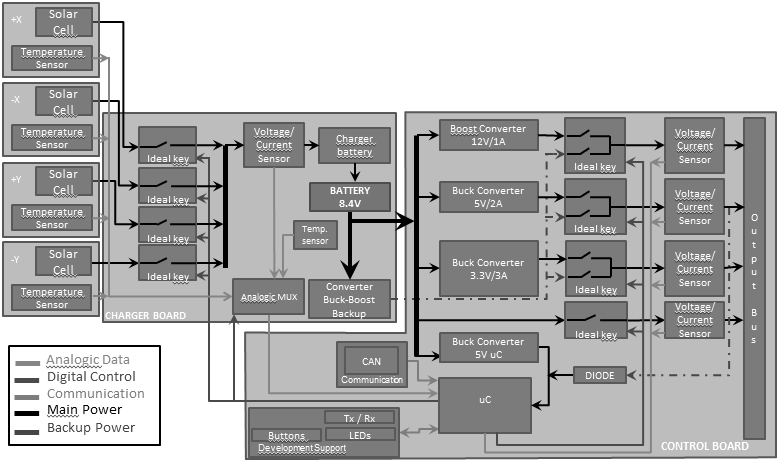
\includegraphics[width=1.0\linewidth]{./figs/diag}
			
		\begin{small}
		Figure \ref{Fig_diag} - Block Diagram. Font: Elaborated by the authors.
		\end{small}		
	\end{figure}
	\pagebreak
	
	%O projeto foi dividido em três partes de desenvolvimento, sendo elas:
	
	%\begin{itemize}
	%\item Painel solar;
	%\item Placa do carregador;
	%\item Placa de controle.
	%\end{itemize}
	
	De maneira simplificada, os painéis solares são responsáveis pela captação da energia solar, convertendo-a em energia elétrica. Essa energia passa para a placa do carregador, passando pelo sistema de carregamento da bateria, passando também por um sensor de tensão e corrente. A energia da bateria tem dois destinos distintos, sendo um deles um conversor backup (que fornece 3,3V, 5V e 12V, podendo fornecer as três tensões ao mesmo tempo) e a placa de controle. 
	
	Na placa de controle existem três conversores de tensão de 12V, 5V e 3,3V, esses conversores são responsáveis por realizar o fornecimento dessas tensões em um barramento de saída, no qual também é possível se obter a tensão diretamente da bateria. Nessa mesma placa está alocado o microcontrolador que possuí um conversor dedicado para a alimentação dele, porém se esse conversor apresentar falha, o barramento de tensão consegue fornecer os 5V para manter o funcionamento do microcontrolador. Entre os conversores e o barramento de saída, existem chaves inteligentes de baixa perdas que fazem um comparativo entre as tensões dos conversores dedicados com o conversor backup e habilita na sua saída o valor que estiver mais confiável. O circuito do conversor backup foi projetado para fornecer sempre um valor pouco inferior aos conversores dedicados, dessa forma as chaves inteligentes por default habilitam sempre os conversores dedicados.
	
	Ainda na placa de controle, existe um microcontrolador para realizar a telemetria do sistema e realizar a comunicação via protocolo CAN com o sistema de computador de bordo. Em caso de alguma falha com esse microcontrolador, o sistema consegue funcionar da maneira desejada, porém sem a  comunicação com a Data Processing Unit.
	
\section{Hardware development}
\label{Hardware development}	

	A seguir será explicado o desenvolvimento do hardware.

\subsection{Solar panel}
\label{Solar panel}

	Para o desenvolvimento do painel solar foram utilizadas fotocélulas de tripla junção (GaInP/GaAs/Ge) do modelo TrisolX Solar Wings, a qual possuí um rendimento de aproximadamente 28\%. Como cada fotocélula consegue fornecer até 2,33V, foi realizado um arranjo com quatro células em série, conseguindo fornecer uma tensão de 9,32V, suficiente para realizar o carregamento da bateria 7,4V de Ion-Lítio utilizada. Foram implementados, em paralelo, seis conjuntos com quatro fotocélulas em série, totalizando 24 fotocélulas no painel solar. Foram utilizados diodos de bypass para evitar danos e perdas de potência do sistema devido a diferenças de características elétricas das fotocélulas, conforme Figure \ref{cells}.
	
	\begin{figure}[th]
		\label{cells}
		\centering
		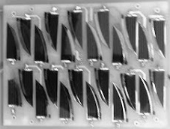
\includegraphics[width=0.9\linewidth]{./figs/cells}
			
		\begin{small}
		Figure \ref{cells} - Solar panel. Font: Picture taken by the authors.
		\end{small}		
	\end{figure}
	\pagebreak
	
\subsection{Charger board}
\label{Charger board}

A placa do carregador é onde está alocado o sistema de carregamento da bateria e o conversor backup, que fornece energia
ao barramento de saída caso ocorra alguma falha no sistema principal, além de contar com um multiplexador analógico que realiza as leituras dos sensores de temperatura dos painéis solares conforme o microcontrolador seleciona o painel desejado.

	\begin{figure}[th]
		\label{charger}
		\centering
		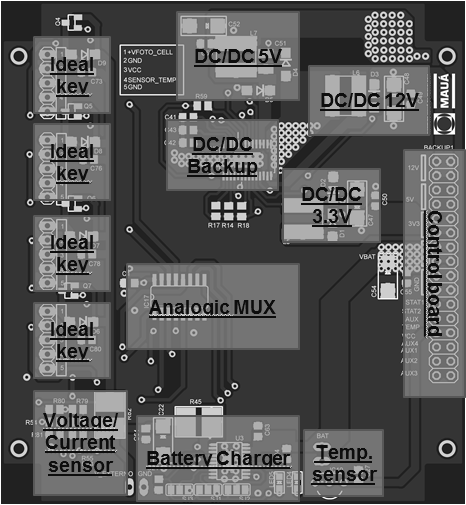
\includegraphics[width=0.9\linewidth]{./figs/charger}
			
		\begin{small}
		Figure \ref{charger} - Charger board. Font: Elaborated by the authors.
		\end{small}		
	\end{figure}


\subsection{Control board}
\label{Control board}

	A placa de controle é responsável pelos conversores principal, chaves inteligentes de baixas perdas e sensores de tensão e corrente, além do microcontrolador que realiza todo o monitoramento do sistema.
	
	\begin{figure}[th]
		\label{control}
		\centering
		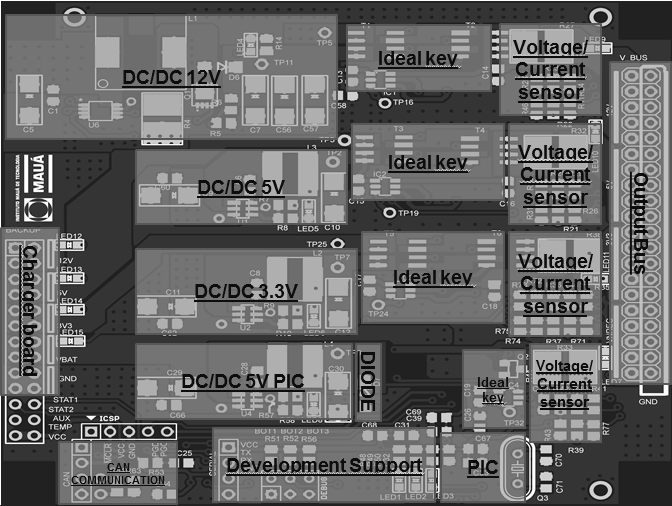
\includegraphics[width=0.9\linewidth]{./figs/control}
			
		\begin{small}
		Figure \ref{control} - Control board. Font: Elaborated by the authors.
		\end{small}		
	\end{figure}

\section{Software development}
\label{Software development}

	Foi desenvolvido um software simples para a realização da telemetria do EPS, que pode ser visualizado de maneira simplificada na Figura \ref{flow}.
	
	\begin{figure}[th]
		\label{flow}
		\centering
		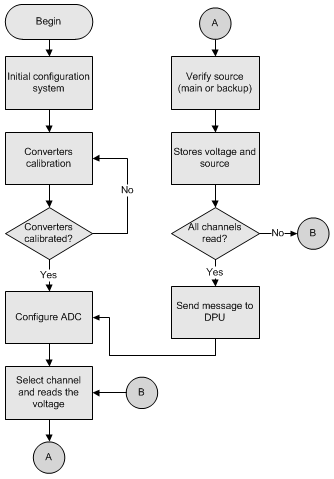
\includegraphics[width=0.8\linewidth]{./figs/fluxo}
			
		\begin{small}
		Figure \ref{flow} - Software flowchart. Font: Elaborated by the authors.
		\end{small}		
	\end{figure}

	A calibração ocorre da seguinte maneira: o microcontrolador força a chave ideal a fornecer o valor da tensão da fonte principal que é armazenada, em seguida o microcontrolador passa a chave ideal para o fornecimento da tensão para o backup e faz um comparativo para validar se o valor da tensão principal é superior ao valor da tensão do backup. Realizando esse ciclo para as três tensões oferecidas no barramento.

\section{Conclusion}
\label{Conclusion}

	 A solução implementada para a aumentar a vida útil do Sistema de Gerenciamento de Energia, utilizando uma fonte \textit{backup} se montou bastante eficaz, o chaveamento entre as fontes de energia principal e \textit{backup} com o uso de chaves ideal se mostrou bastante funcional por apresentar baixa perda e não ocasionar pertubações a carga, que continua operando normalmente. 
	
	O sistema da forma que foi implementado pode se tornar uma plataforma didática para estudos de eletrônica de potência na área aeroespacial, respeitando as normas especificadas pela \textit{Cal Poly}. 

	As redundâncias funcionaram como projetado pelo grupo, fazendo com que caso o conversor principal diminua sua tensão, a ponto de ficar a baixo da tensão fornecida pelo conversor \textit{backup}, este toma seu lugar e começa, imediatamente, a fornecer a energia no barramento de saída, sem que a carga sinta a comutação entre as fontes. Isso ocorre individualmente para cada um dos conversores ou até para todos juntos, não prejudicando o fornecimento de energia aos demais subsistemas do \textit{CubeSat}.

Os tópicos que se destacaram no desenvolvimento do projeto foram:
	
	\begin{itemize}
		\item Alta eficiência atingida com conversores de baixo custo;
		\item Fontes de redundância de alta eficiência;
		\item Chaveamento instantâneo entre fontes;
		\item Utilização de componentes de fácil acesso;
		\item Otimização da área útil do \textit{CubeSat};
		\item Desenvolvimento de \textit{software} supervisório;
		\item Desenvolvimento de um simulador de falhas.
	\end{itemize}


%% The Appendices part is started with the command \appendix;
%% appendix sections are then done as normal sections
%% \appendix

%% \section{}
%% \label{}

%% If you have bibdatabase file and want bibtex to generate the
%% bibitems, please use
%%
%%  \bibliographystyle{elsarticle-harv} 
%%  \bibliography{<your bibdatabase>}

%% else use the following coding to input the bibitems directly in the
%% TeX file.

\begin{thebibliography}{00}

%% \bibitem[Author(year)]{label}
%% Text of bibliographic item

\bibitem[ ()]{}

\end{thebibliography}
\end{document}

\endinput
%%
%% End of file `elsarticle-template-harv.tex'.
